% We switch to portrait mode. This works as advertised.
\documentclass[a0,portrait]{a0poster}
% You might find the 'draft' option to a0 poster useful if you have
% lots of graphics, because they can take some time to process and
% display. (\documentclass[a0,draft]{a0poster})

\usepackage[utf8]{inputenc}

% Switch off page numbers on a poster, obviously, and section numbers too.
\pagestyle{empty}
\setcounter{secnumdepth}{0}

%fonts
\usepackage[T1]{fontenc}
\usepackage[oldstylenums, largesmallcaps]{kpfonts}
\renewcommand*\sfdefault{ugq}

\usepackage{hyperref}
\hypersetup{%
	pdftitle={Effects of a real world size distribution on the heterogeneous crystallisation of hard sphere colloids},%the title
	pdfauthor={Mathieu Leocmach},%your name
}

%proper math and math symbols
%\usepackage{amsmath}
\usepackage{amssymb}

\usepackage{siunitx}

\usepackage{multirow}

% Allow the usage of graphics (.jpg, .png, etc.) in the document
\usepackage{graphicx}
\usepackage{tikz}
\usetikzlibrary{arrows,shapes,backgrounds, positioning, intersections, decorations.markings, decorations.shapes, mindmap, shapes.geometric, matrix, patterns}

\usepackage{pgfplots}
%\usepgfplotslibrary{units}
\usepgfplotslibrary{groupplots}
\pgfplotsset{every axis/.append style={xlabel near ticks,ylabel near ticks}}
\definecolor{BlueViolet}{rgb}{0.62352, 0.372549, 0.623529}

\definecolor{Maroon}{cmyk}{0, 0.87, 0.68, 0.32}
\usepackage{ragged2e}
\RaggedRight
% see documentation for a0poster class for the size options here
\let\Textsize\normalsize
\def\Head#1{\noindent\hbox to \hsize{\hfil{\LARGE\color{Maroon}\raggedright\textothersc{#1}}}\bigskip}
\def\LHead#1{\noindent{\LARGE #1}\smallskip}
\def\Subhead#1{\noindent{\large\textsf{#1}}}
\def\Title#1{\noindent{\VeryHuge\color{Maroon}\raggedright\textothersc{#1}}}

% The textpos package is necessary to position textblocks at arbitary 
% places on the page.
\usepackage[absolute,overlay,%showboxes
]{textpos}
% Set up the grid
%
% Note that [40mm,40mm] is the margin round the edge of the page --
% it is _not_ the grid size. That is always defined as 
% PAGE_WIDTH/HGRID and PAGE_HEIGHT/VGRID. In this case we use
% 15 x 25. This gives us a wide central column for text (7 grid
% spacings) and two narrow columns (3 each) at each side for 
% pictures, separated by 1 grid spacing.
%
% Note however that texblocks can be positioned fractionally as well,
% so really any convenient grid size can be used.
%
\TPGrid[40mm,40mm]{15}{25}  % 3 - 1 - 7 - 1 - 3 Columns

% Mess with these as you like
\parindent=0pt
%\parindent=1cm
\parskip=0.5\baselineskip

\usepackage{paralist}

%bibliography
\usepackage{natbib}
\usepackage{bibentry}
\def\newblock{\hskip .11em plus .33em minus .07em}


%\includeonly{}

\begin{document}
%\tikzset{every mark/.append style={scale=0.8}}
%\pgfplotsset{every axis/.append style={small}}

\bibliographystyle{notitle}
\nobibliography{sift}

% Understanding textblocks is the key to being able to do a poster in
% LaTeX. In
%
%    \begin{textblock}{wid}(x,y)
%    ...
%    \end{textblock}
%
% the first argument gives the block width in units of the grid
% cells specified above in \TPGrid; the second gives the (x,y)
% position on the grid, with the y axis pointing down.

% You will have to do a lot of previewing to get everything in the 
% right place.

% This gives good title positioning for a portrait poster.
% Watch out for hyphenation in titles - LaTeX will do it
% but it looks awful.
\begin{textblock}{15}(0,0)
%\baselineskip=3\baselineskip \Title{
%Effects\,\textit{\Huge of a}\,real world size distribution\\
%\textit{\Huge on the}\,heterogeneous crystallisation\\
%\textit{\Huge of}\,hard sphere colloids\\}
\baselineskip=3\baselineskip \Title{
\begin{tabular}{rl}
Effects\,\textit{\Huge of a} & real world size distribution\\
\textit{\Huge on the} & heterogeneous crystallisation\\
\textit{\Huge of} & hard sphere colloids
\end{tabular}
}
\end{textblock}

\begin{textblock}{11}(0,3)
\LHead{
\begin{tabular}{lp{1.2em}l}
Mathieu Leocmach && \textothersc{Laboratoire de Physique -- UMR 5672,}\\
&& \textothersc{Ecole Normale Supérieure de Lyon}\hfill\texttt{\normalsize mathieu.leocmach@ens-lyon.fr}\\
Hajime Tanaka && \textothersc{Institute of Industrial science, The University of Tokyo}
\end{tabular}
}
\end{textblock}

\begin{textblock}{2.75}(12.20,0.50)
\begin{center}

\includegraphics[width=0.5\columnwidth]{QRcode}\\
\textit{Soft Matter}, 9, 1447--1457 (2013)
\end{center}
\end{textblock}


%Our colloids
\begin{textblock}{3}(4,4.5)
	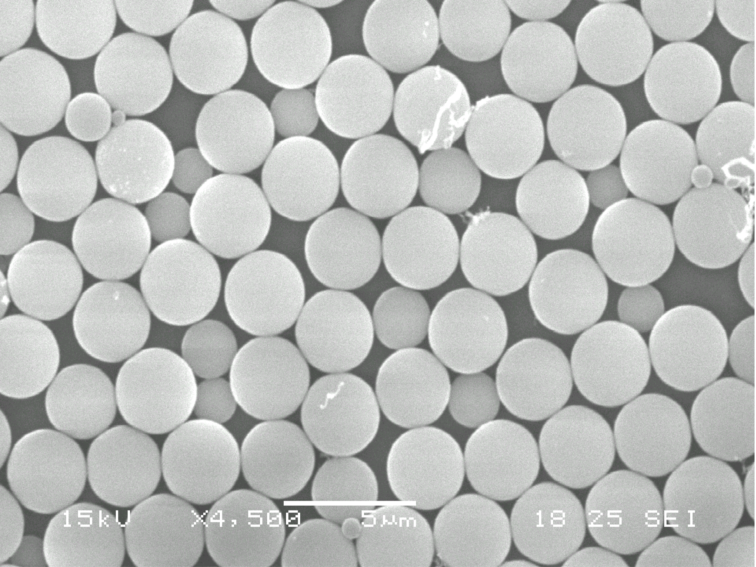
\includegraphics[width=\columnwidth]{SEM.pdf}
	
	\centering
	S.E.M. image
\end{textblock}
\begin{textblock}{3}(0,4.5)
	\Head{Our colloids}
	Index \& density-matched solvent
	\begin{itemize}
		\item Cis-decalin
		\item Cyclohexylbromide
	\end{itemize}
	PMMA particles $\approx$ Hard spheres
	\begin{itemize}
		\item Sterically stabilized
		\item Salt to screen charges\\ (Debye length $<\SI{100}{\nano\metre}$)
	\end{itemize}
\end{textblock}

\begin{textblock}{3}(8,4.5)
	\Head{Size distribution}
	%\tikzset{external/force remake=false}
	\begin{tikzpicture}
	\begin{axis}[%
		name=hist,
		width=0.98\columnwidth, height=0.7\columnwidth,%
		%scale only axis,
		xlabel={Diameters [$\si{\micro\metre}$]},%
		xmin=1, xmax=5,
		axis y line*=left,
		ymin=0, ytick=\empty,%
		ylabel={Size distribution},%
		ylabel near ticks,
		legend style={legend pos=north west}, area legend,
		]
		\addplot[ybar, ybar interval, gray!50, fill=gray!50] file {SEM_size_distrib.txt} \closedcycle;
		\legend{\textsc{sem}}
	\end{axis}
	\begin{axis}[%
		name=hist2,
		width=0.98\columnwidth, height=0.7\columnwidth,%
		xmin=1, xmax=5,
		axis y line*=right,
		ymin=0, ytick=\empty,%
		no marks,%
		]
		\addplot+[dashed] table[x expr ={2*\thisrow{r}}, y=all] {all_ico_icongb_mrco_X.rdist};
		\addlegendentry{In situ};
		\addplot table [x expr ={2*\thisrow{r}/1.25}, y index=1] {all_ico_icongb_mrco_X.rdist};
		\draw[->, ultra thick] (axis cs:3.15,3) -- (axis cs: 3.9, 3) node[midway, above] {swelling};%
	\end{axis}
	\end{tikzpicture}
\end{textblock}

\begin{textblock}{7}(0,8)
	\Head{Single-scale tracking\ldots of polydisperse particles}
	\begin{tikzpicture}
	\begin{groupplot}[%
		group style={
				group name=pics,
				group size=1 by 3,%
				vertical sep=0.1\TPVertModule,
				},%
		anchor=north west,
		width=\TPVertModule,%
		height=\TPVertModule,%
		xmin=0,xmax=64,ymin=0,ymax=64,%
		axis lines=none,%
		scale only axis=true,%
		point meta=explicit symbolic,%
		scatter/@pre marker code/.code={%
        	\pgfmathparse{10*\pgfplotspointmetatransformed*\pgfplotsunitxlength}%
        	%\pgfplotstransformcoordinatex{\pgfplotspointmetatransformed}
            \def\markopts{mark=o,red,mark size=\pgfmathresult}%
            \expandafter\scope\expandafter[\markopts]
            },%
        scatter/@post marker code/.code={\endscope} 
		]
		\nextgroupplot
			\addplot graphics [xmin=0,xmax=64,ymin=0,ymax=64]{not_enough_blur};
			\addplot+[only marks, scatter] table [x index=0, y expr={64-\thisrowno{1}}, meta index=2] {not_enough_blur_centers.txt};
		\nextgroupplot
			\addplot graphics [xmin=0,xmax=64,ymin=0,ymax=64]{good_blur};
			\addplot+[only marks, scatter] table [x index=0, y expr={64-\thisrowno{1}}, meta index=2] {good_centers.txt};
		\nextgroupplot
			\addplot graphics [xmin=0,xmax=64,ymin=0,ymax=64]{too_much_blur};
			\addplot+[only marks, scatter] table [x index=0, y expr={64-\thisrowno{1}}, meta index=2] {too_much_blur_centers.txt};
		\end{groupplot}
	\begin{scope}[text width=1.8*\TPHorizModule]
		\node[right =of pics c1r1] {\Subhead{Not enough blur}\linebreak Mutiple centers};
		\node[right =of pics c1r2] {\Subhead{Enough blur}\linebreak \bibentry{Crocker1996}};
		\node[right =of pics c1r3] {\Subhead{Too much blur}\linebreak Merged centers};
	\end{scope}
	\matrix[matrix of nodes, inner sep=0, anchor=north west] at (4\TPHorizModule,0) (polymono)
	{
	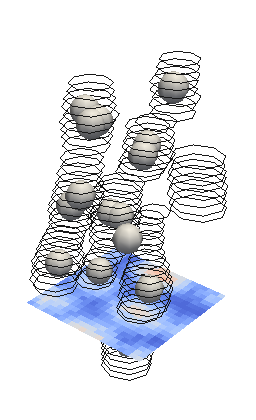
\includegraphics[height=1.5\TPVertModule]{comp3D_monoscale_r20_crop}&
	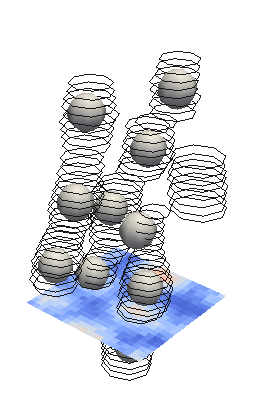
\includegraphics[height=1.5\TPVertModule]{comp3D_monoscale_r25_crop}&
	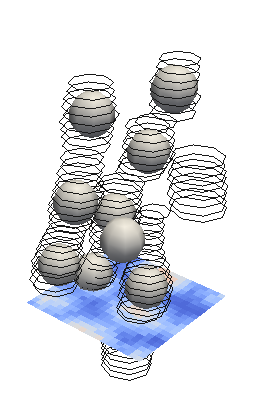
\includegraphics[height=1.5\TPVertModule]{comp3D_monoscale_r30_crop}\\
	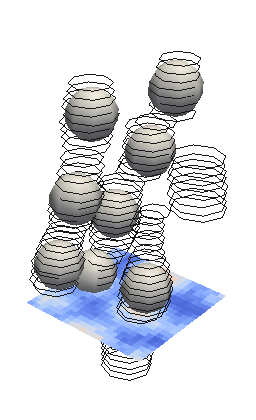
\includegraphics[height=1.5\TPVertModule]{comp3D_monoscale_r35_crop}&
	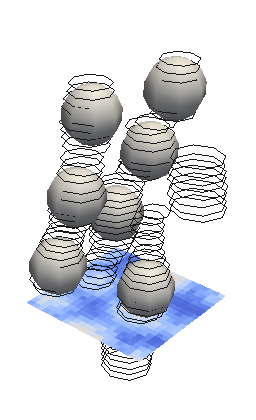
\includegraphics[height=1.5\TPVertModule]{comp3D_monoscale_r40_crop}&
	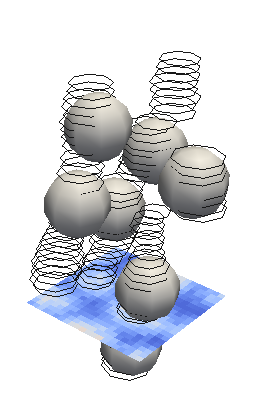
\includegraphics[height=1.5\TPVertModule]{comp3D_monoscale_r45_crop}\\
	};
	%\node[below=-0.5em of polymono]{\Subhead{No good blur}};
	\node[anchor=base] at (polymono.south |- pics c1r3.south) {\Subhead{No good blur}};
	\end{tikzpicture}
\end{textblock}

\begin{textblock}{3}(8,8)
	\Head{Scale space}
	\begin{tikzpicture}[%
		minus/.style={
			shape=circle, draw, inner sep=0, %
			text height=1.5ex,text depth=.25ex,%
			node distance=0.5%
			},%
		]
		\begin{groupplot}[%
			group style={
				group name=toto,
				group size=2 by 1,%
				horizontal sep=0.5\TPHorizModule,
				},%
			anchor=north,%
			width=1.25\TPHorizModule,%
			height=1.25\TPVertModule,%
			xtick=\empty, ytick=\empty,%
			xlabel={position}, xlabel near ticks, ylabel near ticks, %
			no markers,
			title style={%text height=1.5ex,text depth=.25ex, anchor=south, 
			font=\small, text width=1.25\TPHorizModule, align=center},%
			]
			\nextgroupplot[%
				ylabel={intensity},%
				title={Increasing\linebreak Gaussian blur},%
			]
				\addplot[black] table[x expr=\coordindex, y expr=\thisrowno{0}]{gaussians.txt};
				\addplot[blue] table[x expr=\coordindex, y expr=\thisrowno{1}-2]{gaussians.txt};
				\node at (current plot end) (g1) {};
				\addplot[blue!67!red] table[x expr=\coordindex, y expr=\thisrowno{2}-4]{gaussians.txt};
				\node at (current plot end) (g2) {};
				\addplot[blue!33!red] table[x expr=\coordindex, y expr=\thisrowno{3}-6]{gaussians.txt};
				\node at (current plot end) (g3) {};
				\addplot[red] table[x expr=\coordindex, y expr=\thisrowno{4}-8]{gaussians.txt};
				\node at (current plot end) (g4) {};
				
			\nextgroupplot[%
				title={Difference of Gaussians},%
				ymax=0.45,%
			]
				\addplot+[smooth, blue] table[x expr=\coordindex, y expr=\thisrowno{2}-\thisrowno{1}]{gaussians.txt};
				\node at (current plot begin) (DoG1) {};
				\addplot+[smooth, blue!67!red] table[x expr=\coordindex, y expr=\thisrowno{3}-\thisrowno{2}-0.2]{gaussians.txt};
				\node at (current plot begin) (DoG2) {};
				\addplot+[smooth, blue!33!red] table[x expr=\coordindex, y expr=\thisrowno{4}-\thisrowno{3}-0.4]{gaussians.txt};
				\node at (current plot begin) (DoG3) {};
				
		\end{groupplot}
		\node at(0.75\TPHorizModule,0) (O){};

		\node[minus, blue] at (DoG1 -| O) (diff1) {-};
		\draw [->, blue] (g1) -- (diff1);
		\draw [->, blue!67!red] (g2) -- (diff1);
		\draw [->, blue] (diff1) -- (DoG1);
		
		\node[minus, blue!67!red] at (DoG2 -| O) (diff2){-};
		\draw [->, blue!67!red] (g2) -- (diff2);
		\draw [->, blue!33!red] (g3) -- (diff2);
		\draw [->, blue!67!red] (diff2) -- (DoG2);

		\node[minus, blue!33!red] at (DoG3 -| O) (diff3) {-};
		\draw [->, blue!33!red] (g3) -- (diff3);
		\draw [->, red] (g4) -- (diff3);
		\draw [->, blue!33!red] (diff3) -- (DoG3);
		
	\end{tikzpicture}\\
	Magnitude of the DoG maximized at 
	\begin{itemize}
		\item the center of the blob \hfill $\Rightarrow$ \Subhead{position}
		\item the optimal scale  \hfill $\Rightarrow$ \Subhead{size}
	\end{itemize}
	\begin{small}
	\bibentry{Lindeberg1993}\\
	\bibentry{Lowe2004}
	\end{small}
\end{textblock}

\begin{textblock}{3}(12,8)
	\Head{Multiscale tracking}
	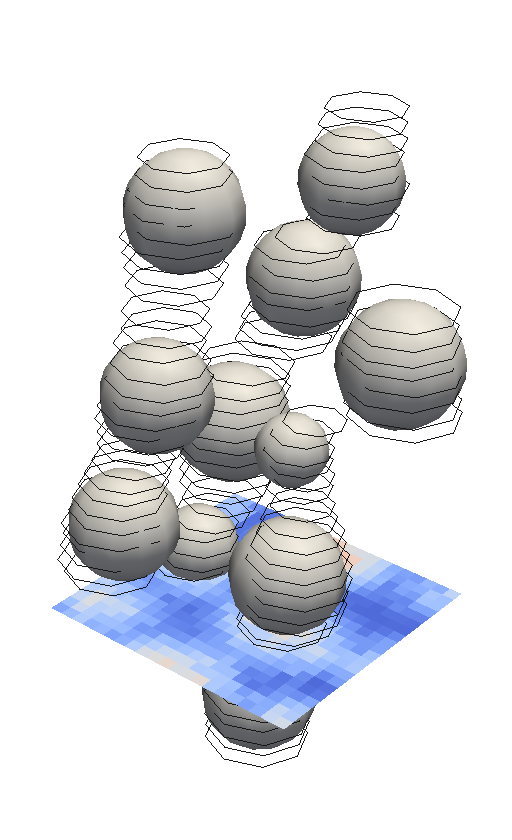
\includegraphics[width=0.5\textwidth]{comp2D3D_crop}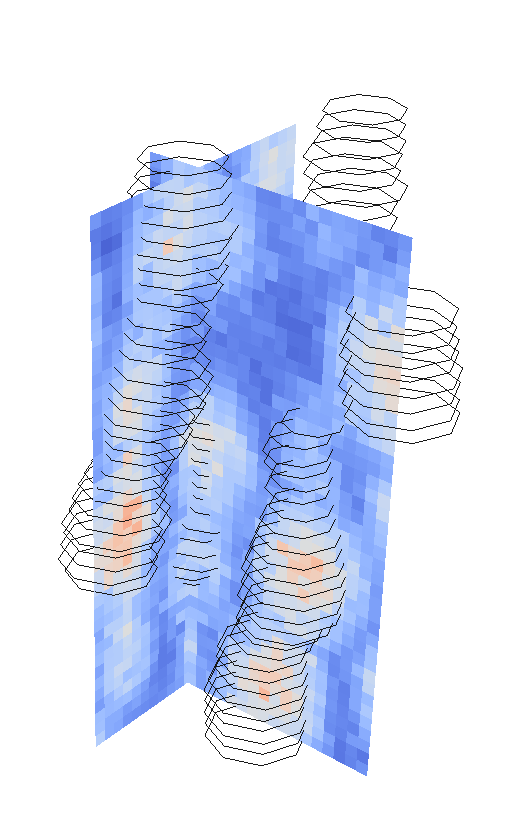
\includegraphics[width=0.5\textwidth]{comp2D3D_slices}
	
	Can track arbitrary size distribution.
\end{textblock}

\begin{textblock}{15}(0,15.35)
	\Head{Layering, Structure visualisation \& Exclusion of small particles}
	\begin{tikzpicture}
		\node[anchor=south east, inner sep=0] at (-0.5\TPHorizModule,0) (t000) {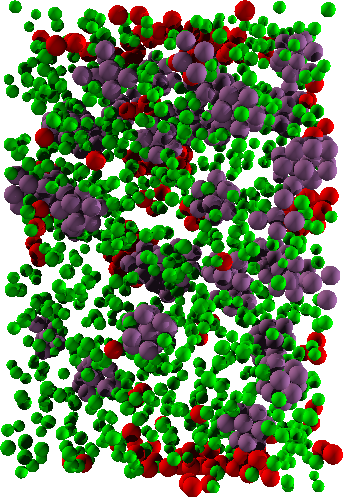
\includegraphics[width=3\TPHorizModule]{mrco_ico_small_t000.png}};
		\node[anchor=south west, inner sep=0] at (0.5\TPHorizModule,0) (t299) {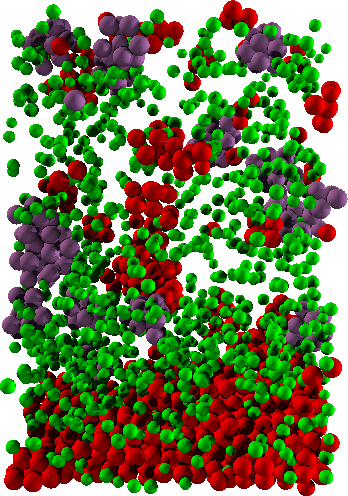
\includegraphics[width=3\TPHorizModule]{mrco_ico_small_t299.png}};
		\node[below right=0 of t000.south west, font=\Large] (a) {$t=0$};
		\draw (a.south east) -- (a.south east -| -7.5\TPHorizModule,0);
		\node[below left=0 of t299.south east, font=\Large] (b) {$t=\SI{40}{\hour}$};
		\draw (b.south west) -- (b.south west -| 7.5\TPHorizModule,0);
		\draw[->, very thick] (0,\TPVertModule) -- (0,3\TPVertModule) node[above]{$z$};
	\end{tikzpicture}
\end{textblock}
\begin{textblock}{4}(0,15.85)
	\begin{tikzpicture}
	\begin{groupplot}[%
			group style={
				group size=2 by 1,
				y descriptions at=edge left,%
				%x descriptions at=edge bottom,%
				horizontal sep=0.2\TPHorizModule,
			},%
			width=1.7\TPHorizModule,
			height=5\TPVertModule,%
			xmin=0, xmax=1,%
			xtick={0,0.2,...,1},%
			no marks,%
			xlabel={$\rho$},
			xlabel near ticks,%
			ylabel=$z/(2R_\text{peak})$,%
			ymin=1, ymax=26,%
			axis on top,
			reverse legend,
			legend style={
				at={(1,0.75)}, anchor=east,%
				font=\footnotesize,
				text width=0.65\TPHorizModule,		
				}
			]
		\nextgroupplot
		\addlegendimage{empty legend}
		\addlegendentry{(smoothed)}
		\addplot+[gray!50, fill=gray!50,area legend] table[x index=1, y index=0]{large_small_mrco_t000.gauss.zhist} -- (rel axis cs:0,1) \closedcycle;
		\addlegendentry{Large}
		\addplot+[dashed, red, very thick] table[x index=3, y index=0]{large_small_mrco_t000.gauss.zhist};
		\addlegendentry{Crystal-like}
		\addplot+[black] table[x index=1, y index=0]{large_small_mrco_t000.zhist};
		\addlegendentry{Large}

		\nextgroupplot[xmax=0.2, xtick={0,0.1,0.2}]
		\addlegendimage{empty legend}
		\addlegendentry{(smoothed)}
		\addplot+[gray!50, fill=gray!50,area legend] table[x index=2, y index=0]{large_small_mrco_t000.gauss.zhist} -- (rel axis cs:0,1) \closedcycle;
		\addlegendentry{Small}
		\addplot+[dashed, red, very thick] table[x index=3, y index=0]{large_small_mrco_t000.gauss.zhist} ;
		\addlegendentry{Crystal-like}
		\addplot+[black] table[x index=2, y index=0]{large_small_mrco_t000.zhist};
		\addlegendentry{Small}
		\end{groupplot}
	\end{tikzpicture}
\end{textblock}


\begin{textblock}{3.75}(11.25,15.85)
	\begin{tikzpicture}
	\begin{groupplot}[%
			group style={
				group size=2 by 1,
				y descriptions at=edge right,%
				%x descriptions at=edge bottom,%
				horizontal sep=0.2\TPHorizModule,
			},%
			width=1.7\TPHorizModule,
			height=5\TPVertModule,%
			xmin=0, xmax=1,%
			xtick={0,0.2,...,1},%
			no marks,%
			xlabel={$\rho$},
			xlabel near ticks,%
			ylabel=$z/(2R_\text{peak})$,%
			ymin=1, ymax=26,%
			axis on top,
			reverse legend,
			legend style={
				at={(1,0.75)}, anchor=east,%
				font=\footnotesize,
				text width=0.65\TPHorizModule,		
				}
			]
		\nextgroupplot
		\addlegendimage{empty legend}
		\addlegendentry{(smoothed)}
		\addplot+[gray!50, fill=gray!50] table[x index=1, y index=0]{large_small_mrco_t200.gauss.zhist} -- (rel axis cs:0,1) \closedcycle;
		\addlegendentry{Large}
		\addplot+[dashed, red, very thick] table[x index=3, y index=0]{large_small_mrco_t200.gauss.zhist};
		\addlegendentry{Crystal-like}
		\addplot+[black] table[x index=1, y index=0]{large_small_mrco_t200.zhist};
		\addlegendentry{Large}
		

		\nextgroupplot[xmax=0.2, xtick={0,0.1,0.2}]
		\addlegendimage{empty legend}
		\addlegendentry{(smoothed)}
		\addplot+[gray!50, fill=gray!50] table[x index=2, y index=0]{large_small_mrco_t200.gauss.zhist} -- (rel axis cs:0,1) \closedcycle;
		\addlegendentry{Small}
		\addplot+[dashed, red, very thick] table[x index=3, y index=0]{large_small_mrco_t200.gauss.zhist} ;
		\addlegendentry{Crystal-like}
		\addplot+[black] table[x index=2, y index=0]{large_small_mrco_t200.zhist};
		\addlegendentry{Small}
		\end{groupplot}
	\end{tikzpicture}
\end{textblock}

\begin{textblock}{3}(0,12.1)
	\Head{Buoyancy control}
	\Subhead{by temperature control}
	\begin{itemize}
	\item Find $T_\text{matching}$ (a few days)
	\item $T>T_\text{matching}$
	\begin{itemize}
		\item makes particles sink
		\item melts the crystals at the top
	\end{itemize}
	\item Back to $T_\text{matching}$
	\end{itemize}
	$\Rightarrow$ observe at the top crystallisation from the beginning.
\end{textblock}

\begin{textblock}{7}(4,12.1)
	\Head{Size distributions within local structures}
	\begin{center}
	\begin{tikzpicture}
	\begin{groupplot}[%
		group style={
			group name=distrib,
			group size=2 by 1,
			horizontal sep=\TPHorizModule,
			},%
		width=3\TPHorizModule,%
		height=2\TPHorizModule,%
		no marks,%
		xlabel={$R$ [$\si{\micro\metre}$]}, xmin=0.8, xmax=2.5,%
		ylabel={Size distribution}, ymin=0, ymax=12, ytick=\empty,%
		legend style={legend pos=north west},
		]
		\nextgroupplot
		\addplot[gray!50,fill=gray!50, area legend] table[x=r, y=all] {all_ico_icongb_mrco_X.rdist} \closedcycle;
		\addplot[dashed,red] table[x=r, y=mrco] {all_ico_icongb_mrco_X.rdist};
		\addplot[brown, very thick] table[x=r, y=X] {all_ico_icongb_mrco_X.rdist};
		\legend{all, crystal-like, crystalline};
		
		\nextgroupplot
		\addplot[gray!50,fill=gray!50, area legend] table[x=r, y=all] {all_ico_icongb_mrco_X.rdist} \closedcycle;
		\addplot[dashed,blue] table[x=r, y=ico] {all_ico_icongb_mrco_X.rdist};
		\addplot[BlueViolet, very thick] table[x=r, y=icongb] {all_ico_icongb_mrco_X.rdist};
		\legend{all, ico. centre, ico. surf.};
	\end{groupplot}
	\end{tikzpicture}
	\end{center}
\end{textblock}

\begin{textblock}{3}(12,12.1)
	\Head{Local structures}
	Identified using bond orientational order\\
	\begin{footnotesize}
	\begin{itemize}
	\item \bibentry{steinhardt1983boo}
	\item \bibentry{Lechner2008}
	\item \bibentry{Leocmach2012}
	\end{itemize}
	\end{footnotesize}
	
	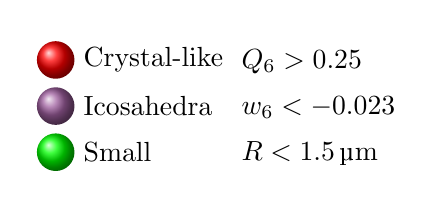
\begin{tikzpicture}
		\matrix[%
		matrix of nodes, ampersand replacement=\&,
		column 3/.style={right, text height=0.8em, text depth=0.2em},%
		column 2/.style={right},
		column 1/.style={left, circle, shade, inner sep=0.4\baselineskip},%
		] (l)
	{
		|[ball color=red]|{} \& Crystal-like \& $Q_6>0.25$\\
		|[ball color=BlueViolet]|{} \& Icosahedra \& $w_6<-0.023$\\
		|[ball color=green]|{} \& Small \& $R<\SI{1.5}{\micro\metre}$\\
	};
	\end{tikzpicture}
\end{textblock}


\begin{textblock}{15}(0,21.5)
	\Head{Heterogeneous nucleation, Exclusion of small particles \& Formation of grain boundaries}
	\begin{tikzpicture}
	\node[%
		fill=gray!25, minimum width=\TPVertModule, minimum height=14.25\TPHorizModule,%
		single arrow, single arrow head extend=0.25\TPVertModule,%
		%anchor=west,
		] (arrow) {};
	\matrix[%
		matrix of nodes, inner sep=1pt, column sep=0.25\TPHorizModule,%
		%row 3/.style={text width=2\TPHorizModule, align=center}%
		] (a)%
		{%
			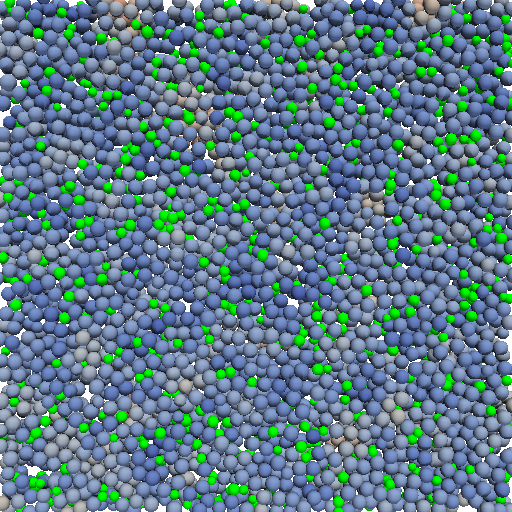
\includegraphics[width=2\TPHorizModule]{small_boo000.png} & %
			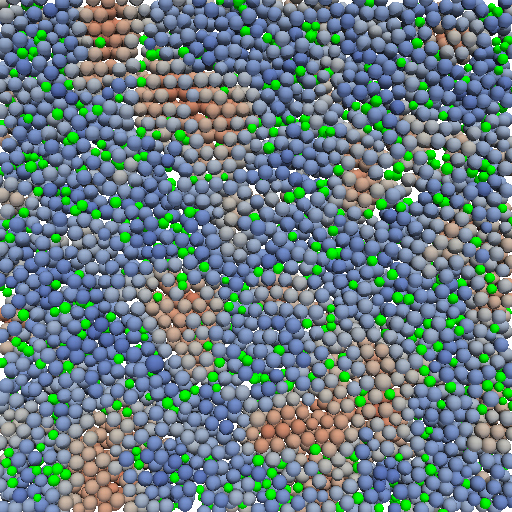
\includegraphics[width=2\TPHorizModule]{small_boo060.png} & %
			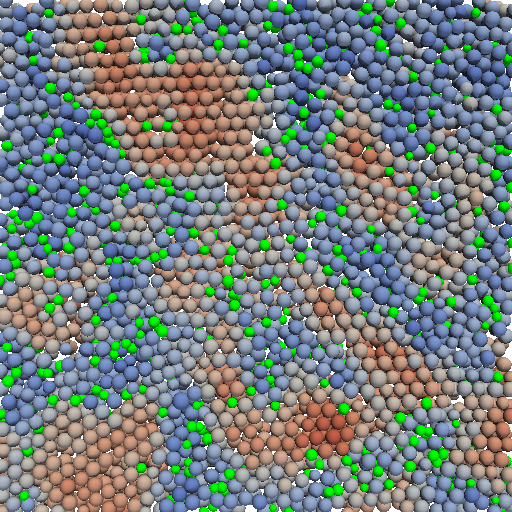
\includegraphics[width=2\TPHorizModule]{small_boo120.png} &
			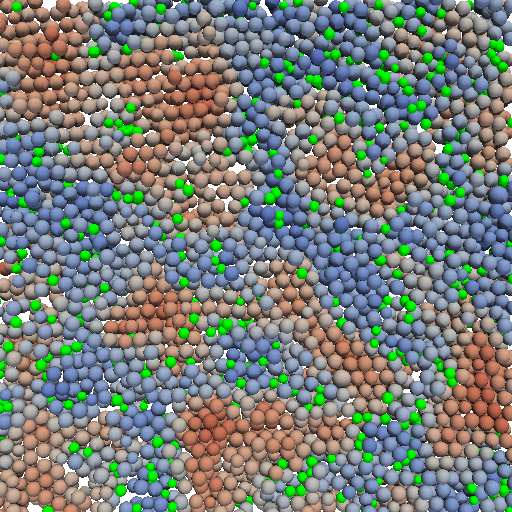
\includegraphics[width=2\TPHorizModule]{small_boo180.png} & %
			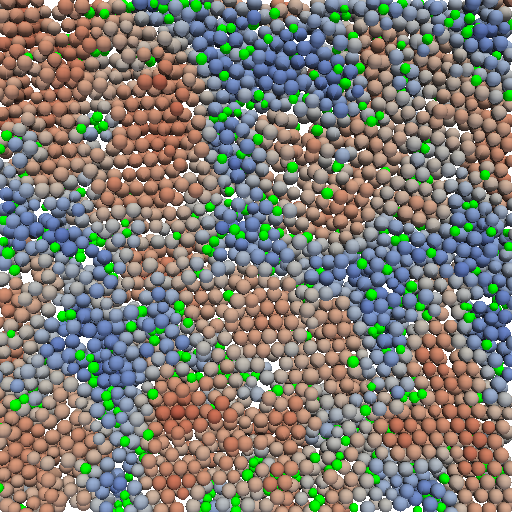
\includegraphics[width=2\TPHorizModule]{small_boo240.png} & %
			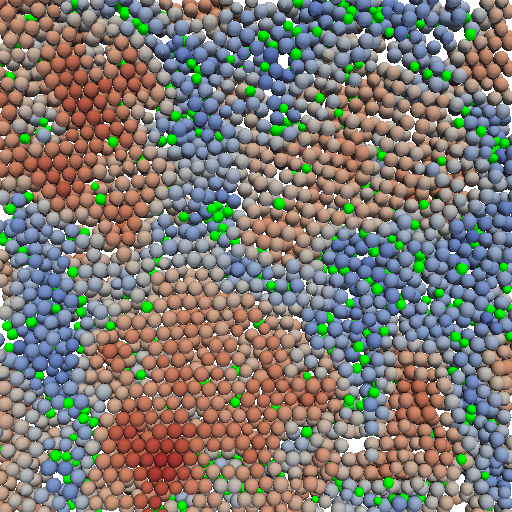
\includegraphics[width=2\TPHorizModule]{small_boo299.png}\\%
			$0$ & \SI{12}{\hour} & \SI{24}{\hour} & \SI{36}{\hour} & \SI{48}{\hour} & \SI{60}{\hour}\\
		};
		\node[above right=0 of a-1-1.north west] {$Q_6$ fluctuations constrained by small particles};
		\node[above right=0 of a-1-3.north west] {Crystal nucleate in high $Q_6$ fluctuations};
		\node[above right=0 of a-1-5.north west] {Small particles are expelled and form grain boundaries};
		\begin{axis}[%
		name=b,
		at={(arrow.tail)},%
		anchor=east,%
		xmin=0,xmax=10, ymin=0, ymax=0.55,%
		width=0.5\TPHorizModule,%
		height=2\TPVertModule,%
		axis x line=none,%
		axis y line*=left,%
		axis on top,
		]
		\addplot graphics[xmin=0,xmax=10, ymin=0, ymax=0.55] {color_bar.png};
		\end{axis}
		\node[above= 0 of b.outer north] {$Q_6$};
	\end{tikzpicture}
\end{textblock}

\textblockcolour{lightgray!50!white}
\TPMargin*{ 0.125\TPHorizModule }
\begin{textblock}{2.875}(12,3.125)%real width of 3
	\Head{Take away}
	\Subhead{A reliable method to}
	\begin{itemize}
		\item track particles even when
		\begin{itemize}
			\item arbitrary size distribution
			\item high density
		\end{itemize}
		\item measure the sizes
		\begin{itemize}
			\item of each particles
			\item in situ
		\end{itemize}
	\end{itemize}
	\Subhead{Small particles}
	\begin{itemize}
		\item promote icosahedral order for a size ratio of 0.8
		\item must be expelled before crystal-like ordering
		\item induce polycrystalline material
	\end{itemize}
	
	%\textsf{The crystal is important} to understand the glass.
\end{textblock}%Conclusion



\end{document}